%% bare_jrnl_compsoc.tex
%% V1.4a
%% 2014/09/17
%% by Michael Shell
%% See:
%% http://www.michaelshell.org/
%% for current contact information.
%%
%% This is a skeleton file demonstrating the use of IEEEtran.cls
%% (requires IEEEtran.cls version 1.8a or later) with an IEEE
%% Computer Society journal paper.
%%
%% Support sites:
%% http://www.michaelshell.org/tex/ieeetran/
%% http://www.ctan.org/tex-archive/macros/latex/contrib/IEEEtran/
%% and
%% http://www.ieee.org/

%%*************************************************************************
%% Legal Notice:
%% This code is offered as-is without any warranty either expressed or
%% implied; without even the implied warranty of MERCHANTABILITY or
%% FITNESS FOR A PARTICULAR PURPOSE! 
%% User assumes all risk.
%% In no event shall IEEE or any contributor to this code be liable for
%% any damages or losses, including, but not limited to, incidental,
%% consequential, or any other damages, resulting from the use or misuse
%% of any information contained here.
%%
%% All comments are the opinions of their respective authors and are not
%% necessarily endorsed by the IEEE.
%%
%% This work is distributed under the LaTeX Project Public License (LPPL)
%% ( http://www.latex-project.org/ ) version 1.3, and may be freely used,
%% distributed and modified. A copy of the LPPL, version 1.3, is included
%% in the base LaTeX documentation of all distributions of LaTeX released
%% 2003/12/01 or later.
%% Retain all contribution notices and credits.
%% ** Modified files should be clearly indicated as such, including  **
%% ** renaming them and changing author support contact information. **
%%
%% File list of work: IEEEtran.cls, IEEEtran_HOWTO.pdf, bare_adv.tex,
%%                    bare_conf.tex, bare_jrnl.tex, bare_conf_compsoc.tex,
%%                    bare_jrnl_compsoc.tex, bare_jrnl_transmag.tex
%%*************************************************************************


% *** Authors should verify (and, if needed, correct) their LaTeX system  ***
% *** with the testflow diagnostic prior to trusting their LaTeX platform ***
% *** with production work. IEEE's font choices and paper sizes can       ***
% *** trigger bugs that do not appear when using other class files.       ***                          ***
% The testflow support page is at:
% http://www.michaelshell.org/tex/testflow/


\documentclass[10pt,conference,onecolumn,compsoc]{IEEEtran}


\usepackage{hyperref}
\usepackage{enumitem}
\setlist[itemize]{leftmargin=3 cm}
\setlist[enumerate]{leftmargin=3cm}



% *** CITATION PACKAGES ***
%
\ifCLASSOPTIONcompsoc
  % IEEE Computer Society needs nocompress option
  % requires cite.sty v4.0 or later (November 2003)
  \usepackage[nocompress]{cite}
\else
  % normal IEEE
  \usepackage{cite}
\fi
% cite.sty was written by Donald Arseneau
% V1.6 and later of IEEEtran pre-defines the format of the cite.sty package
% \cite{} output to follow that of IEEE. Loading the cite package will
% result in citation numbers being automatically sorted and properly
% "compressed/ranged". e.g., [1], [9], [2], [7], [5], [6] without using
% cite.sty will become [1], [2], [5]--[7], [9] using cite.sty. cite.sty's
% \cite will automatically add leading space, if needed. Use cite.sty's
% noadjust option (cite.sty V3.8 and later) if you want to turn this off
% such as if a citation ever needs to be enclosed in parenthesis.
% cite.sty is already installed on most LaTeX systems. Be sure and use
% version 5.0 (2009-03-20) and later if using hyperref.sty.
% The latest version can be obtained at:
% http://www.ctan.org/tex-archive/macros/latex/contrib/cite/
% The documentation is contained in the cite.sty file itself.



% *** GRAPHICS RELATED PACKAGES ***
%
\ifCLASSINFOpdf
   \usepackage[pdftex]{graphicx}
 
\else
 
\fi
% graphicx was written by David Carlisle and Sebastian Rahtz. It is
% required if you want graphics, photos, etc. graphicx.sty is already
% installed on most LaTeX systems. The latest version and documentation
% can be obtained at: 
% http://www.ctan.org/tex-archive/macros/latex/required/graphics/
% Another good source of documentation is "Using Imported Graphics in
% LaTeX2e" by Keith Reckdahl which can be found at:
% http://www.ctan.org/tex-archive/info/epslatex/
%
% latex, and pdflatex in dvi mode, support graphics in encapsulated
% postscript (.eps) format. pdflatex in pdf mode supports graphics
% in .pdf, .jpeg, .png and .mps (metapost) formats. Users should ensure
% that all non-photo figures use a vector format (.eps, .pdf, .mps) and
% not a bitmapped formats (.jpeg, .png). IEEE frowns on bitmapped formats
% which can result in "jaggedy"/blurry rendering of lines and letters as
% well as large increases in file sizes.
%
% You can find documentation about the pdfTeX application at:
% http://www.tug.org/applications/pdftex









% *** PDF, URL AND HYPERLINK PACKAGES ***
%
\usepackage{url}
% url.sty was written by Donald Arseneau. It provides better support for
% handling and breaking URLs. url.sty is already installed on most LaTeX
% systems. The latest version and documentation can be obtained at:
% http://www.ctan.org/tex-archive/macros/latex/contrib/url/
% Basically, \url{my_url_here}.




\begin{document}

\title{Spitfire '91, a WPF Shmup}
%
%

% received ..."  text while in non-compsoc journals this is reversed. Sigh.

\author{Victor Gasior and Jaxx 'Lucky' Woods
}

\IEEEtitleabstractindextext{%
\begin{abstract}
Spitfire '91 is a retro inspired Shoot 'em Up game (or shmup) where you control a small airplane fighting drones, tanks, and enemy aircraft. The target audience for this project is fans of retro schups like EDF or UN Squadron. So far we have constructed just the basic plans for the project.
\end{abstract}

}


% make the title area
\maketitle



\IEEEdisplaynontitleabstractindextext

\IEEEpeerreviewmaketitle



\section{Introduction}
Spitfire '91 should be a fun, fast paced, retro inspired Shoot 'em Up game made in WPF / C Sharp. In Spitfire '91 the player controls a modern military fighter jet and fights enemy jets, drones, and ground vehicles. The game is supposed to emulate an SNES (Super Nintendo Entertainment System) era Shoot 'em Up game with its own art, design, sounds, and mechanics. There will be at least one stage where the players can fight enemies in order to try to get a higher and higher high scores. The target audience for this game will be Shoot 'em Up enthusiasts and fans of retro styled video games in general. The audience should first and foremost enjoy the game, while also tailoring the experience to resemble a retro shmup without making it difficult for fans of modern video games to enjoy.  There are not many Shoot 'em Up games produced any more so we are appealing to a niche audience starved of content.

% needed in second column of first page if using \IEEEpubid
%\IEEEpubidadjcol


\subsection{Background}
Shoot em' Ups rely on a player controller a vehicle that can move around the screen and shoot enemies that are trying to attack the player. The player obtains score by avoiding and defeating enemies. The game ends once they reach the end of the level / stage or loses do to being hit by enemies too many times

The reason we decided to undertake this project is that Shoot 'em Ups are both fun to play, and seem interesting to design.

\subsubsection{Important Terminology}
Shump - Common abbreviation for Shoot 'em Up
High Score - A goal of a Shoot 'em Up game, players try to earn higher scores.

\subsection{Impacts}
This game should bring enjoyment to the audience and provide a free modern alternative to old retro Shoot 'em Up games that can be hard to play due to old hardware and games not being ported to modern systems.

\subsection{Challenges}
Handling enemy, projectile, and player collision in WPF.
Displaying information and moving backgrounds in WPF.
Storing enemy and level data in WPF.


\section{Scope}
This game should the bare minimum contain one playable level with multiple enemy variations that can spawn. There should be a win and lose state, as well as a connected 'Game Over' screen on loss. There should be a main menu screen the user accesses first before starting the main game. There should be a high score tracker which displays and saves the highest scores to add replay value. Current Stretch Goals are as follows: multiple levels with different backgrounds, a working, upgrade shop and currency system, game saving, and music

\subsection{Requirements}
The requires come from how we intend the game to operate, and what we think will be the most fun for the user to experience. The requirements both make it so the game is operational (i.e. game actually works, core elements, etc. ), while also trying to make the user experience as great as possible. (i.e. sound and visual effect feedback)

\subsubsection{Functional}
\begin{itemize}
\item User needs to be able to control the character to avoid enemies and shoot enemies.
\item User needs to be able to earn points by eliminating enemies.
\item User needs to be able to view their current score.
\item Game needs to spawn enemies for the player to both avoid and shoot.
\item User needs to be able to lose, then be able to try again.
\end{itemize}

\subsubsection{Non-Functional}
\begin{itemize}
\item There should be visual effects and sound effects to enhance the game experience.
\item There should be a scrolling background to give the user the impression of flying

\end{itemize}

\subsection{Use Cases}
 \ref{tab:useCaseIndex}.




\begin{table}
\centering
\begin{tabular}{|c|c|c|c|c|}
\hline
Use Case ID & Use Case Name & Primary Actor & Complexity & Priority \\
\hline \hline
1 & Play Game & user & High & 1\\
\hline
2 & Check Highscore & user & Med & 2\\
\hline
3 & Pause Game & user & Easy & 3\\
\hline
\end{tabular}
\caption{Sample use case table}
\label{tab:useCaseIndex}
\end{table}


\begin{itemize}
\item[Use Case Number:] 1
\item[Use Case Name:] Playing the Game
\item[Description:] A user wants to play the game, they will open the game and hit 'play' on the main menu.
\end{itemize}

\begin{enumerate}
\item User opens the application.
\item User hits play.
\item User plays the game until loss.
\item[Termination Outcome:] The user's score is saved, highest score is updated if this score is the new highest score, which is displayed on the main menu. 
\end{enumerate}

\begin{itemize}
\item[Use Case Number:] 2
\item[Use Case Name:] Check Highscore
\item[Description:] A user wants to check the highscore of the local game.
\end{itemize}

\begin{enumerate}
\item User opens the application.
\item[Termination Outcome:] The user looks at the score on the main menu.
\end{enumerate}


\begin{itemize}
\item[Use Case Number:] 3
\item[Use Case Name:] Pausing the Game
\item[Description:] A user wants to pause the game during use
\end{itemize}

\begin{enumerate}
\item User is currently playing the game.
\item User pauses the game using the 'p' key
\item[Termination Outcome:] The user keeps the game paused for as long as they want, unpausing if they wish by hitting 'p' again
\end{enumerate}


\subsection{Interface Mockups}
At first, this will largely be completely made up, as you get further along in your project, and closer to a final product, this will typically become simple screenshots of your running application.

In this subsection, you will be showing what the screen should look like as the user moves through various use cases (make sure to tie the interface mockups back to the specific use cases they illustrate).

\begin{figure}[ht!]
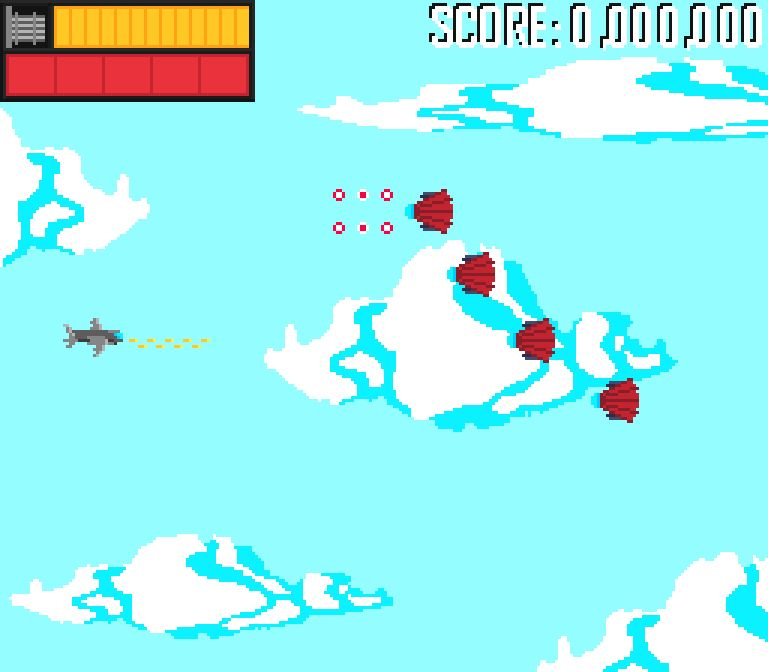
\includegraphics[height=250px, width=350px]{Spitfire_91MockUp.jpg}
\caption{This displays an idea for how the game looks during play}
\label{cat1}
\end{figure}


\section{Project Timeline}
We have already made a basic prototype, but we have yet to develop the minimum viable product to show to the class. The steps we will take to create the project will go as follows: 
1. Create a game engine that will control several important functions such as: Movement control, enemy spawning, and collision detection.
2. Create the movement controls and projectile firing. 
3. Create the spawning of enemies and allow several different versions of enemies to be selected. This includes making an abstract enemy object and its concrete children.
4. Create the system of collision detection. This also controls the losing of health and gaining of points as certain collisions are detected. 
5. Create a Game Over state and display the appropriate state for a game over.
6. Create a Pause Function 
7. Create a main menu with High Score Board.
8. Polishing Audio and Visual presentation.

\section{Project Structure}
The project switches between three main windows, that open and close as appropriate. The Main Menu, is exactly what you would think it is, it has the controls for starting and exiting the game as well as displaying the highest scores. The GameMain is what controls the game and is what the player will spend most of their time in. This window is switches to GameOverWindow upon the player losing the game. The GameOverWindow allows the player to go straight to either the GameMain or MainMenu window, as well as displaying the score the player just achieved.


\subsection{UML Outline}
\ref {UML}
Here you can see the UML for our program. The meat of the program is in the GameEngine class, that contains several important functions that are called by both the game's main window 'GameMain' and the GameOverWindow. The Bullet class is derived from the bullet template (Template Design Pattern) and provides the fireBullet function the Rectangle it needs to add to the screen. The spawnEnemy function needs an Enemy class, including EnemyBasic and it's two children (Factory Design Pattern). The three windows are designed to be swapped between when certain functions are called.
\begin{figure}[ht!]
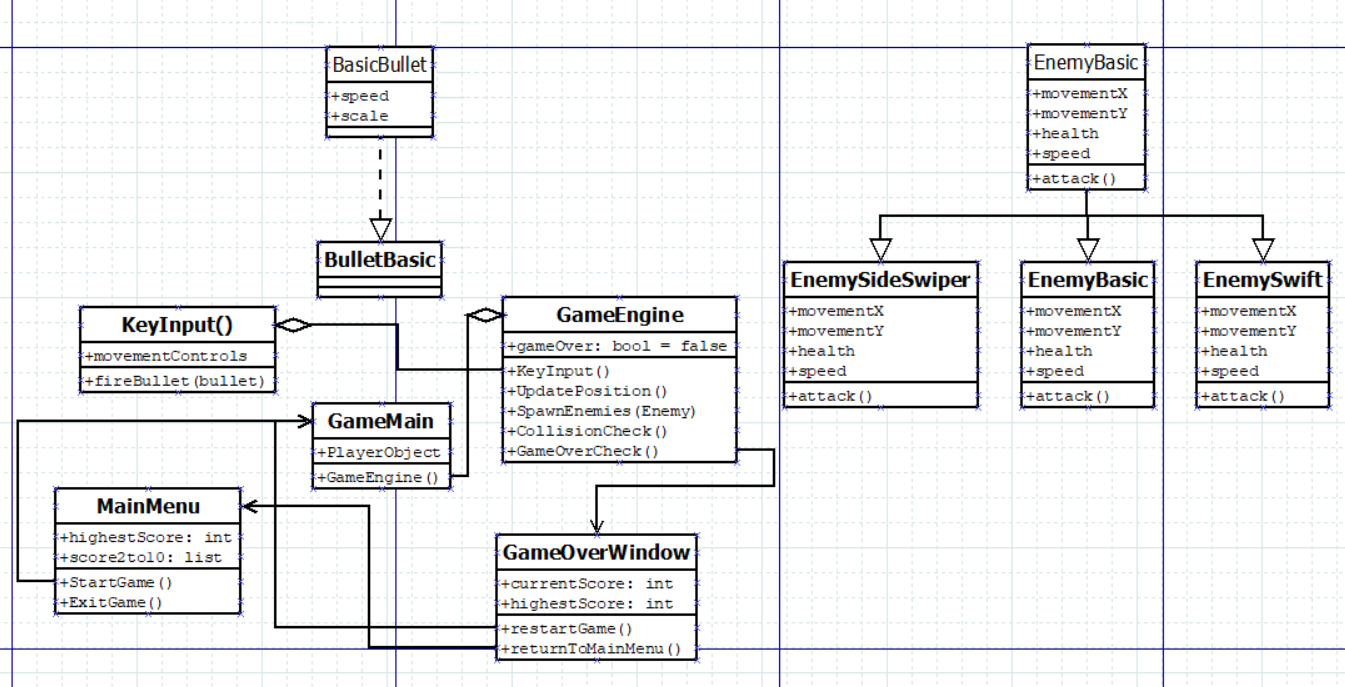
\includegraphics[height=250px, width=350px]{DIA.png}
\caption{This is the UML}
\label{UML}
\end{figure}

\subsection{Design Patterns Used}
We are implementing the Factory Pattern and Template Pattern for the project.


\section{Results}
Turns out WPF is not really meant for making games, and by not really, we mean not at all. WPF is an absolute nightmare to make games for, causing us to have to find weird workarounds and use things in strange unintended ways. Since neither of us took any graphics classes before hand we were stuck wrangling with the default WPF canvas. Currently we got a 'game' where you can move around the plane and shoot, but not much else. As it currently stands, enemy spawning is currently broken, and without enemy spawning various game functions like health, scoring, and the game over screen have no function.

\subsection{Future Work}
We are about $\frac{3}{5}^{ths}$ done with the project, but we only have so much time left. Highest priority is getting enemies to work, as without enemies key functions of the game like scoring have no purpose or function. We also need to make the Main Menu and Game Over menu, including the saving and displaying of high scores.





% that's all folks
\end{document}

